\section{Эксперименты}

В этой главе сначала будет дано детальное описание наборов данных, применяемых в рассматриваемой задаче. Далее будут описаны ключевые метрики, используемые для оценки качества моделей. В заключение будут представлены эксперименты и проведено сравнение полученных результатов работы исследуемых архитектур графовых нейронных сетей.

\subsection{Описание используемых наборов данных}

В качестве данных для обучения и тестирования моделей используются наборы отзывов на товары и отели с ресторанами на сайтах-агрегаторах Amazon и Yelp. Впервые их применили в работе CARE-GNN \cite{dou2020}. Выбор обусловлен распространенностью для оценки среди исследований по определению мошенничества, а также большим объемом и реальным, а не искусственным происхождением.

В данных Amazon содержится информация о 12 тыс. людях, среди которых 1.1 тыс. (9.5\%) являются мошенниками, и 4.4 млн. связях между ними. Отзывы собраны с подраздела сайта о музыкальных инструментах, причем пользователь помечался недоброжелателем, если его рецензии получали положительную оценку от других пользователей в менее чем 20\% случаев. Для исследования предоставлено 25 характеристик, а пользователей объединяли связями трех типов:

\begin{enumerate}
    \item U-P-U -- оставили отзыв об одном и том же продукте.

    \item U-S-V -- имели одинаковый рейтинг в течение недели.

    \item U-V-U -- наивысшие 5\% сходства текста отзывов на один и тот же товар, что измеряли с помощью алгоритма term frequency, inverse document frequency (TF-IDF).
\end{enumerate}

Данные Yelp содержат 46 тыс. отзывов на рестораны и отели, среди которых 6.6 тыс. (14.5\%) обозначены как мошеннические. Общее количество связей в наборе составляет 3.9 млн, представлено 32 характеристики, а рецензии объединяли по следующим признакам:


\begin{enumerate}
    \item R-U-R -- отзывы, опубликованные одним и тем же пользователем.

    \item R-S-R -- под одним и тем же местом, с одинаковым рейтингом.

    \item R-T-R -- под одним и тем же рестораном или отелем, опубликованы в одном месяце.
\end{enumerate}

Таким образом, выбранные наборы данных позволяют решать задачи как определения мошеннических отзывов, так и выявления самих недоброжелателей. При этом простая структура позволяет легко представить данные в виде графа или таблицы, в зависимости от используемой модели.

Стоит отметить, что в работах часто используются и другие наборы, часто из банковской сферы. Например, Bank Account Fraud \cite{jesus2022} представляет собой 6 млн. записей и 30 признаков, сгенерированных на основе реальных финансовых данных открытия счетов. В другом примере, Credit Card Fraud \cite{pozzolo2015}, авторы собрали 285 тыс. реальных транзакций и обработали их 30 характеристик с помощью метода Principal Component Analysis (PCA).  Однако проблема таких данных заключается в их синтетическом (то есть искусственном) происхождении, из-за невозможности раскрыть персональную информацию. Это усложняет интерпретацию и может привести к ухудшению качества обучения модели при использовании на реальных задачах."

\pagebreak



\subsection{Метрики}

Неверный выбор метрик для оценки может исказить полученные выводы, потому важно учесть все особенности данных. В случае поставленной задачи, наборы Amazon и Yelp являются достаточно несбалансированными, то есть содержат всего 9.5\% и 14.5\% пользователей-мошенников и их отзывов из всех данных соответственно. Учитывая это, для  оценки исследуемых решений будут использоваться следующие две метрики:

\begin{enumerate}

    \item F1-мера (f1-score):

\begin{equation}
    \text{F1-score} = 2 \cdot \frac{\text{Recall} \cdot \text{Precision}}{\text{Recall} + \text{Precision}} = \frac{\text{TP}}{\text{TP} + \frac{\text{FP} + \text{FN}}{2}}
\end{equation}
где полнота -- \(\text{Recall} = \frac{\text{TP}}{\text{TP} + \text{FN}}\), точность -- \(\text{Precision} = \frac{\text{TP}}{\text{TP} + \text{FP}}\) оценивают способность модели находить все примеры и точно их отмечать, а F1-мера соответсвует их среднему гармоническому. TP (true positive) и TN (true negavite) соответствуют числу верно найденных моделью 1 и 0 соответственно, а FP (false positive) и FN (false negative) -- ее ошибкам. 

    \item Площадь по кривой (Area Under Curve, AUC): равна доле пар объектов вида (классы 1 и 0), которые модель верно упорядочила, то есть предсказанная вероятность на первом больше:

\begin{equation}
    \operatorname{AUC} = \frac{\sum \limits_{i=1}^{N} \sum \limits_{j=1}^{N} \mathbb{I} [y_i < y_j] I^{\prime}[f(x_{i}) < f(x_{j})]}{\sum \limits_{i=1}^{N} \sum \limits_{j=1}^{N} \mathbb{I} [y_i < y_j]}
\end{equation}

\begin{equation}
    I^{\prime}\left[f(x_{i}) < f(x_{j})\right]=
    \left\{
      \begin{array}{ll}
        0, & f(x_{i}) > f(x_{j}) \\
        0.5, & f(x_{i}) = f(x_{j}) \\
        1, & f(x_{i}) < f(x_{j})
      \end{array}
    \right.
\end{equation}

\begin{equation}
    \mathbb{I} \left[ y_{i}< y_{j} \right]=
    \left\{
      \begin{array}{ll}
        0, & y_{i} \geq y_{j} \\
        1, & y_{i} < y_{j}
      \end{array}
    \right.
\end{equation}
\end{enumerate}

Полученную формулу AUC можно также представить как площадь под графиком, где по оси X отложена доля ложноположительных объектов, а по оси Y -- доля верноположительных.

Выбранные метрики учитывают непропорциональность классов в данных, так как они усредняют разные отношения верно и неверно предсказанных объектов в каждом классе.

\pagebreak



\subsection{Эксперименты}

Для выбора наилучшей архитектуры графовой нейронной сети в рамках данной работы были проведены эксперименты, в ходе которых протестированы основные расмотренные ранее подходы с различными структурными компонентами. Число выбранных работ невелико в связи с ограничениями имеющихся вычислительных мощностей.

Код реализации нейронных сетей написан на языке программирования Python с использованием таких библиотек, как PyTorch и PyG для создания основных компонентов, DGL для работы с графовыми данными, WandB для наглядного сохранения результатов экспериментов и другими. Все метрики и итоговый программный код можно найти в репозиторях, соответствующих названиям архитектур: \href{https://github.com/qw1zzard/CARE-GNN}{CARE-GNN}, \href{https://github.com/qw1zzard/antifraud}{GTAN}, \href{https://github.com/qw1zzard/GAGA}{GAGA} и \href{https://github.com/qw1zzard/DRAG}{DRAG}, а графики -- в общем \href{https://wandb.ai/qw1zzard-wandb?shareProfileType=copy}{WandB проекте}.

Сначала наборы отзывов и данных о пользователях сайтов загружаются и преобразуются согласно требованиям соответствующего подхода. Например, в DRAG \cite{kim2023} ко всем узлам добавляется петля для дальнейшего нахождения полного внимания (self-attention). Затем они делятся на выборки для обучения, валидации и тестирования соответственно, после чего начинается этап тренировки, в котором используются следующие параметры:

\begin{enumerate}
    \item CARE-GNN: 40\% данных в обучающей выборке, остальные в тестовой; 30 эпох, lr = 0.01, \(\lambda_1\) = 2, \(\lambda_2\) = 0.001, размер пакета = 1024 и применение субдискретизации.

    \item GTAN: 40\% в тестовой части, 15 эпох, lr = 0.003, 128 записей в пакете, \(\lambda_2\) = 0.0001, 2-хслойная нейросеть, 5 групп обучения и использование исключения.

    \item GAGA: 40\% данных в тренировочной выборке, 50\% в тестовой и 10\% в валидационной; 500 эпох, lr = 0.001, 256 и 512 -- размеры пакетов в Amazon и Yelp соответственно, 2 слоя нейросети, глубина hop-4, применение исключения и 4 головы внимания.

    \item DRAG: 10\% записей в обучающей, 23\% в валидационной и 67\% в тестовой выборке; 1000 эпох, lr = 0.01, 1024 записей в пакете, \(\lambda_2\) = 0.001 и 8 голов обучения.
\end{enumerate}
где эпоха -- это полный проход алгоритма по всем данным, lr -- параметр, отвечающий за скорость обучения; \(\lambda_1\) и \(\lambda_2\) (сокращение весов, weight decay) -- параметры регуляризации, размер пакета (batch size) отвечает за число записей в одном шаге обучения, субдискретизация (undersampling) применяется для исправления несбалансированности классов, группы обучения (folds) делят данные на несколько частей для большей устойчивости процесса тренировки модели, а исключение (dropout) отключает часть весов случайным выбором для лучшей обобщающей способности. Это список основных параметров, применяемых во всех работах, но есть и дополнительные, например, награды (rewards) при обучении с подкреплением в CARE-GNN \cite{dou2020}.

{
    \centering
    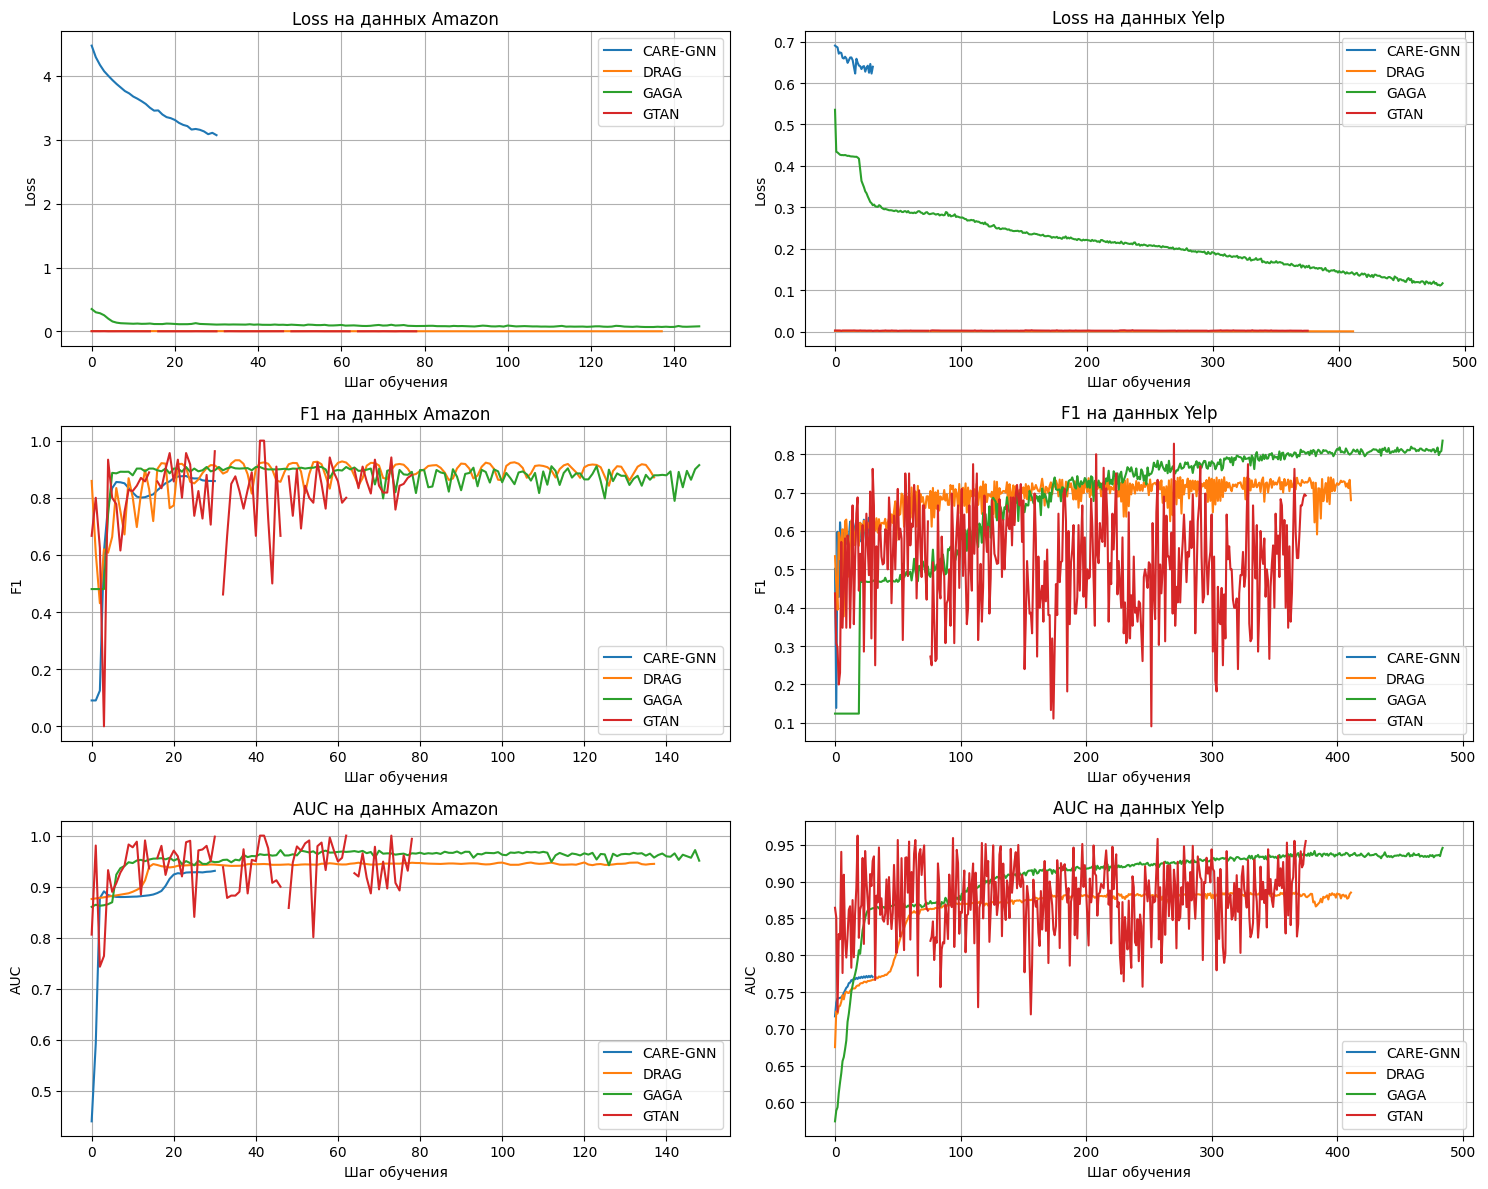
\includegraphics[width=1.05\linewidth]{images/experiments.png}
    \captionof{figure}[experiments]{Значения функции потерь (loss), f1-меры и площади под кривой на данных Amazon и Yelp соответственно.}
    \label{experiments}
}

Всего для сравнения на двух наборах было обучено 4 модели. Был проведен анализ производительности, включая сравнение времени обучения и использования ресурсов.

Из графиков на рис.~\ref{experiments} видно, что самая ранняя работа CARE-GNN имеет меньше всего шагов обучения и остается на уровне значения функции потерь сильно хуже других. У данной архитектуры наименьшие требования к ресурсам, что, вероятно, могло быть вызвано ограничениями на момент выхода статьи.

Модели DRAG \cite{kim2023} и GAGA \cite{wang2023} имеют больше всего шагов обучения и стальное снижение значения функции потерь при росте метрик с каждым шагом. Плато обучения достигается примерно к 350-й итерации, что можно рассматривать как момент, когда можно прекратить тренировку модели без значительной потери качества.

Графики F1-меры и AUC у модели GTAN \cite{xiang2023} имеют стохастический вид, так как в ней применяется разбиение обучающей выборки на 5 групп, в каждой из которых один пакет содержит только 128 записей. Таким образом, обучение приобретает неоднозначный характер, когда сложно сказать, в какой именно момент тренировка закончилась и началось переобучение.

\pagebreak



\subsection{Сравнение результатов}

Лучшие метрики были зафиксированы в ходе тестирования рассмотренных моделей на валидационной выборке для каждого набора данных. Все работы прошли тренировочный процесс независимо три раза, а затем были взяты усредненные значения полученных оценок и времени обучения.

\begin{center}
    \begin{longtable}{|l|c|c|c|c|c|c|}
    \caption{Полученные усредненные метрики моделей на валидации. Здесь все величины представлены в процентах для лучшей читаемости, а время обучения обозначено как число минут : секунд.} \\ \hline

    \multicolumn{1}{|c|}{\textbf{Наборы данных}} & \multicolumn{3}{c|}{\textbf{Amazon}} & \multicolumn{3}{c|}{\textbf{Yelp}} \\ \hline

    \textbf{Модель} & \textbf{F1-мера} & \textbf{AUC} & \textbf{Время} & \textbf{F1-мера} & \textbf{AUC} & \textbf{Время} \\ \hline

    CARE-GNN & 85.69 & 92.03 & 2:49 & 61.01 & 77.06 & 11:10 \\ \hline

    GTAN & \textbf{91.58} & \textbf{95.56} & 10:28 & 75.57 & 89.24 & 5:47 \\ \hline

    GAGA & 91.36 & 95.13 & \textbf{0:28} & \textbf{83.34} & \textbf{94.50} & \textbf{5:31} \\ \hline

    DRAG & 89.03 & 94.30 & 5:42 & 68.71 & 87.25 & 16:02 \\ \hline

    \noalign{\global\arrayrulewidth=1.5pt}  \hline
    \noalign{\global\arrayrulewidth=.4pt}

    NGS & 92.28 & 97.36 & -- & 78.28 & 92.18 & -- \\ \hline

    GCN & 65.71 & 81.89 & -- & 49.63 & 55.04 & -- \\ \hline

    GAT & 53.90 & 74.26 & -- & 52.28 & 55.19 & -- \\ \hline

    GraphSAGE & 83.83 & 91.49 & -- & 57.81 & 74.09 & -- \\ \hline
    \end{longtable}
\end{center}

Из результатов видно, что среди рассмотренных моделей GAGA с подходом разделения соседей по классам перед агрегацией показала наилучшую оценку на наборе данных Yelp при наименьшем среднем времени обучения. Выделяются также метрики упомянутой ранее работы NGS \cite{qin2022}, однако авторы не предоставили исходный код для воспроизведения своих исследований, что затрудняет проверку результатов.

На данных Amazon лучше всего себя показала модель GTAN. Таким образом, обе работы, использующие GAT \cite{velickovic2017} в качестве ключевого модуля и с акцентом на проблеме гетерогенных графов, получили наилучшие оценки. Это указывает на значительную эффективность внимания в обработке таких данных и подтверждает значимость подхода в решении подобных задач.

В дополнение, в таблице представлены оценки оригинальных GCN \cite{kipf2017}, GAT и GraphSAGE \cite{hamilton2017} соответственно. Видно, что трансформерный и спектральный подходы в данной задаче проявили себя особенно плохо, а пространственный, наоборот, без дополнительных модификаций и доработок получает сравнительно хорошие оценки.

В целом, полученные метрики коррелируют со временем обучения и масштабами моделей, что явно позволяло им лучше справляться с рассмотренными задачами. При этом набор данных Yelp, содержащий отзывы на рестораны и отели, более сложную задачу для всех архитектур. Вероятно, наилучшим подходом для него может быть использование трансформерной модели непосредственно к тексту рецензии, возможно, даже без представления исходных данных в виде графовой структуры.

\pagebreak
